\chapter{System}

The purpose of this chapter is to introduce the System in more details, Overall we are using for this work a Python script. The library  used in this work are: Request,JSON,Os,Subprocess,Getpass,Sys,Urllib3.
The use of the The Request library was for creating the interaction with the Web services of XNAT. The Python Requests library is the go-to solution for making HTTP requests in Python, thanks to its elegant and intuitive API that simplifies the process of interacting with web services and consuming data in the application.\footnote{https://www.datacamp.com/tutorial/python-subprocess} The sys module in Python provides access to variables and functions that interact closely with the Python interpreter and runtime environment. 

The fact that a JSON command is written the use of the JSON library was necessary. JSON is a syntax for storing and exchanging data.it a text, written with JavaScript object notation.\footnote{schoolW3, Phython JSON}
The Python subprocess module is a tool that allows to run other programs or commands from your Python code. Using the Python subprocess module is like giving commands to your computer using Python instead of typing them directly into the command prompt. This module makes it easy to automate the Python code.\footnote{https://www.datacamp.com/tutorial/python-subprocess}. Getpass() prompts the user for a password without echoing. The getpass module provides a secure way to handle the password prompts where programs interact with the users via the terminal.\footnote{https://www.geeksforgeeks.org/python/getpass-and-getuser-in-python-password-without-echo/}
 The import of urllib3 was to disable the InsecureRequestWarning, which is normally shown when requests connects to a site with an unverified SSL certificate. This approach helps keep the output clean and free of unnecessary warnings during the run of the Script.
 Currently the System is running Docker Engine 28.3.0,The Docker Client version in use is 20.10.5+dfsg1, which communicates with the Docker Engine to issue commands and manage images and containers. The XNAT web application is running on version 1.9.1.1, as verified through the web interface. 
 

\begin{figure}
    \centering
    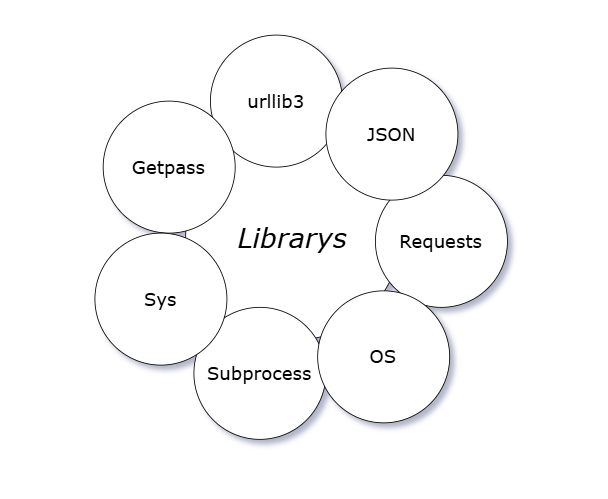
\includegraphics[width=0.7\linewidth]{en/content/lp.png}
    \caption{Schema: Core Libraries for Python Scripting in System Integration }
    \label{fig:enter-label}
\end{figure}


\section{Architecture and organization of the Code:}
 The automation script is structured into 17 distinct parts, each responsible for a specific step in the overall workflow.
 During the development of the automation script, i closely followed the steps of the manual process, since I had already tested and completed it manually. I carefully repeated the same steps during the implementation. In other words in every structured part is composed from a function that is responsible of doing a step of the manual Process.
 
 \section{The Dockerfile:}
 
The first function is responsible for writing the dockerfile, the function is called \texttt{def write\_dockerfile} and it takes three arguments the target directory for the dockerfile, the name of the Python script to include, and an optional base Docker image (defaulting to python:3.10-slim, currently the fastest and the slimest image of docker). The function creates the necessary folder (if it doesn't already exist), constructs the Dockerfile content, and writes it. The content of the dockerfile is introduced with a string interpolation and it containts the base image and numerous commands like WORKDIR /app (A working directory ) \texttt{COPY \{script\_filename\} /app/\{script\_filename\}} to copy the user skript inside of the image. The line  RUN pip install \texttt{--no-cache-dir pandas} tells Docker to install the pandas Python library using pip during the build process of the Docker image.  which helps reduce the overall image size and avoids unnecessary layers in the building process. The last component of the dockerfile is the \texttt{COPY requirements.txt /app/requirements.txt}, in this part it gives the opportunity for the user to write in a separate text file all the libraries used in the container script, which can be used later in the image build process.
i removed the CMD instruction from the Dockerfile because it caused errors when running the container in XNAT. The issue was due to a conflict between the CMD instruction in the Dockerfile and the command.json configuration, as both included the python3 prefix. This led to a duplicate command execution, which caused the container to fail. By removing CMD in the Dockerfile, the execution logic is now fully controlled by XNAT through the command.json, ensuring proper behavior during container launch.

\begin{lstlisting}[language=bash]
FROM python:3.10-slim
WORKDIR /app
COPY script.py /app/script.py
RUN pip install --no-cache-dir pandas
COPY requirements.txt /app/requirements.txt
\end{lstlisting}
The rest of the \texttt{def write\_dockerfile} ensures that the specified directory exists, then creates and writes a Dockerfile to that location.It constructs the full path to the file, writes the generated content into it, prints a confirmation message.


\lstset{
  language=Python,
  basicstyle=\ttfamily\small\color{black},
  keywordstyle=\color{black},
  identifierstyle=\color{black},
  stringstyle=\color{black},
  commentstyle=\color{black},
  numberstyle=\color{black},
  showstringspaces=false
}

\begin{lstlisting}
os.makedirs(docker_dir, exist_ok=True)
dockerfile_path = os.path.join(docker_dir, "Dockerfile")
with open(dockerfile_path, "w") as f:
    f.write(dockerfile_content)
print(f"Dockerfile written to {dockerfile_path}")
return dockerfile_path
\end{lstlisting}

This function ensure that the dockerfile will be written in a appropriate way and it secures that all the dependencies are stored in the external requirement text file. It handles all possible cases and avoid the issues of errors and the Stdin errors. 

\section{Building, Pushing and Tagging the image :}

when a command is deployed in XNAT and a container is being launched, the first thing that XNAT is controlling if the docker image is available in the DockerHub. Which means the user has to have essentially a account in the Docker hub, and preferably to log himself before using the following script.  consequently its essential to push and tag the image created.
The function responsible for the build is the \texttt{def build\_docker\_image}. and its expecting two parameters: 
\texttt{dockerfile\_path } for the Dockerfile path and the the name/tag for the Docker image to be built \texttt{docker\_image\_name}. For the build we used subprocess.run to call the external docker build command.
usually when we want to build an image in docker we use the basic command \texttt{docker built  .} 


\begin{lstlisting}
 build_result = subprocess.run(["docker", "build", "-f", dockerfile_path, "-t", docker_image_name, "."],  capture_output=True, text=True)
    if build_result.returncode != 0:
        print(f"Build failed:\n{build_result.stderr}")
        sys.exit(1)
\end{lstlisting}

As we can see in this block it showing  subprocess.run was used  to call the external docker build command and the -f ,dockerfile\_path, tells Docker which Dockerfile to use.The  -t ,docker\_image\_name, sets the name and tag for the image. The point (.) at the end of the command means the current directory will be used as the build context. In addition the \texttt{capture\_output=True} collects both stdout and stderr so the script can handle their output or errors, and the text=True makes sure outputs are returned as strings.
\\Now that the image has been succesfully built we can proceed  to the next essential Step:  "pushing the image to Docker Hub". In order to do that the same method by building of \texttt{subprocess.run} is used.


\begin{lstlisting}
full_tag = f"{dockerhub_username}/{docker_image_name}"
print(f"Pushing image to Docker Hub as '{full_tag}'...")
    push_result = subprocess.run(["docker", "push", full_tag], capture_output=True, text=True)
    if push_result.returncode != 0:
        print(f"Push failed:\n{push_result.stderr}")
        sys.exit(1)

\end{lstlisting}

In normal cases we use the comamnd \texttt{docker push the imagename}, and this assumes that the user is already logged in to their Docker account. However, in the automation script we make use of the \texttt{subprocess.run}. 
To explain this block,we begin by discussing the reason for using the full tag image. It constructs a full image tag in the Docker Hub format. Since the Docker Hub need image tags  to be in the format: The full image tag follows the format \texttt{dockerhub\_username/image\_name[:tag]}.

This line creates a correctly formatted name for your Docker image, so it links your Docker Hub account \texttt{(dockerhub\_username)} with the chosen image and optional version tag \texttt{(docker\_image\_name)}.

The line of the code: 
\begin{lstlisting}
push_result = subprocess.run(["docker", "push", full_tag], capture_output=True, text=True)
\end{lstlisting}
refers to the push process with the \texttt{subprocess.run} methode. And it follows the same concept as builing the Docker image. 

\section{The Prompt Function for the required input:}

 This function performs the task of capturing input from the user.
 We have used this function in the script in multiple scenarios. First of them to take the Docker Hub user name from the user, in order to customize the JSON command we asked the user about the name of the Command and her description, And overall, it is used to take the username and password from the user's login credentials.The function proceeds through all of this steps by running the script.
 The function looks like this:
 
 \begin{lstlisting}
 def get_input(prompt):
    while True:
        value = input(prompt)
        if value.strip():
            return value
        else:
            print("Cannot be empty.")

\end{lstlisting}
The \texttt{ def get\_input} uses a while True loop to keep asking until the user enters a input, the \texttt{value.strip()} removes any whitespace from the user input.If the input is valid the value is returned, if it not the \texttt{Cannot be empty} will be printed.


\section{The JSON Command :}

To communicate to XNAT the docker image, and consequently to run the container in the Web site. it is necessary to write a JSON Command. 
\footnote{https://wiki.xnat.org/container-service/json-command-definition}
Usually the JSON command is personalized and customized depending on the main idea of the image. But in the automation case the JSON command must be custumized for all the cases, which means no matter which file is  selected still the command will handle it.
To achieve that the function used called \texttt{create\_json\_file},which builds the configuration dictionary for a Docker-based XNAT command (for the XNAT container service), writes it to a command.json file, and returns the filename.
The function expect three parameters:
\texttt{docker\_image} The Docker image to use (string),\texttt{script\_filename} The name of the Python script inside the container (string), \texttt{ mod\_data} :A dictionary holding user-provided metadata (names, descriptions, etc.)
Lets start analyzing the first block of the JSON command:
\begin{lstlisting}

json_file = {
        "name": mod_data["command_name"],
        "description": mod_data["command_description"],
        "version": "1.5",
        "type": "docker",
        "image": docker_image,
        "command-line": f"python3 /app/{script_filename} /input/#input_file# /output",
        "mounts": [
            {"name": "input", "path": "/input", "writable": False},
            {"name": "output", "path": "/output", "writable": True}
        ],
\end{lstlisting}


In this block we are  defining the name of the Command, add a description and specify the version and the type of the image.
The command line declares the actual command to run inside of the container when invoked by XNAT. The placeholder \# is a template substitution (not a Regex Expression)  that tells XNAT \texttt{ "When you launch the Docker command, replace \#input\_file\# with the actual file name/path that the user selected as input."}, it does not define what a valid file looks like. It marks a spot in the command where XNAT should "fill in" an actual value.

The mount configures the directory mappings (as Docker Volume) between XNAT and the Docker container. Most of the time two are used, the input and the output.
we specified the Path: "/input" in the container and if the container can write or just read the files  \texttt{Not writable or Writable}.

The second part of the JSON Command:


\begin{lstlisting}

 "inputs": [
            {
                "name": "input_files",
                "description": "Input files",
                "type": "files",
                "element_type": "file",
                "required": True,
                "mount": "input",
                "multiple": True
            }
        ],
        "outputs": [
            {
                "name": "result_file",
                "type": "file",
                "description": "Result file output",
                "mount": "output",
                "path": "."
            }
        ],
\end{lstlisting}


This block defines the parameters that a user must provide as a input file when launching the container. 
Let's break down each field:\\

the \texttt{The "name": "input\_files"}  This name is used in other parts of the JSON in references—such as placeholders in the command-line. In addition we add a optional human friendly description. The type means that the input accepts more than a file, not just text files or scans or numbers, and we specify that each elelment in the input is specifficaly a file with  the \texttt{"element"}.
The required \texttt{= true} is mainly to refer that if the input is not provided the command can not be run. The mount in this part links the input to a specific mount inside of the container. All files provided by the user will appear in the /input directory inside the container. With the \texttt{multiple : True} its indicated that the user can upload or select more than one file for this input.
The same logic applies for the output part the only point that needed to be referred to it more is the \texttt{"path": "."} and this means the output file will be in the top level of the \/output directory. and it allows more than one output file, use "type": "files" in the output block.

The final block in the Command JSON :

\begin{lstlisting}

 "xnat": [
            {
                "name": wrapper_name,
                "label": mod_data["label_name"],
                "description": mod_data["label_description"],
                "contexts": ["xnat:projectData"],  
                "external-inputs": [
                    { 
                        "name": "project",
                        "type": "Project",
                        "required": True,
                        "load-children": True
                    }
                ],
                "output-handlers": [
                    {
                        "name": "output",
                        "accepts-command-output": "result_file",
                        "as-a-child-of": "project",
                        "type": "Resource",
                        "label": "Results",
                    }
\end{lstlisting}

This block defines what will be displayed on the XNAT interface and it connects the docker command with XNAT's web interface and permission system. It controls how the command appears as a tool in XNAT, how it integrated with projects or other data and how input are handled.
The wrapper name is the technical name of the command inside XNAT, the \texttt{"label": mod\_data["label\_name"]} is a human-readable name shown in XNAT UI. The \texttt{"description": mod\_data["label\_description"]} is a description for the tool/wrapper, shown when users browse tools in XNAT. For the context it referees where we want to appear the container in the interface of XNAT, since the main idea was to have one Container on top of the structure of XNAT, here \texttt{["xnat:projectData"]}means this command is available at the project level.
 In the external input external entities from XNAT are defined. The fact that we used Project as a context for the command, concequently we require in the external input a projct to be selected, in more details the name and the type must be Project. This input must be provided that why \texttt{True} is written.
 We tell the XNAT with \texttt{"load-children": True:} to load load (in the UI) the child objects of the project when showing this input.\\
 In the output-handlers part we control  how the outputs from your command are stored and shown in XNAT after job completion.\\
 This output-handler tells XNAT to take the result file the command produces, store it as a resource under the project, call that section “Results” in the UI. 
 The \texttt{as-a-child-of": "project"} reffers that the results are uploaded in XNAT project back as new recources.

 Finally the script writes the JSON Command file, ensuring that the JSON Command is saved in a correct format ready to be uploaded in XNAT.
 
 \section{Upload the Command in XNAT:}

 After writing the JSON command the next step is to send it to XNAT, and to achieve this we have to use the appropriate REST API responsible for uploading the container Command in XNAT.
 We can find the list of all REST APIS under the \texttt{Administer->Site Administration->Miscelianous->Development Utilities->Swagger} .
 To send the Command to XNAT we found that the responsible REST API for it is POST.\footnote{https://xnat-dev.gwdg.de/xapi/swagger-ui.html\#/command-rest-api}
 The function responsible for that is the \texttt{def send\_json\_to\_xnat} and it expecting four parameters: \texttt{json\_file\_path, xnat\_url, xnat\_user, xnat\_password}. Working with REST APIS we have to proceed at first with building the URL Endpoint for XNAT’s command registration.
 
\begin{lstlisting}
def send_json_to_xnat(json_file_path, xnat_url, xnat_user, xnat_password): 

    url = f"{xnat_url}/xapi/commands"
    print(f"Uploading command to {url}")
    with open(json_file_path, "r") as f:
        response = requests.post(url, auth=(xnat_user, xnat_password), json=json.load(f))
    if response.status_code == 200:
        print("Command uploaded successfully.")
    elif response.status_code == 201:
        print("Command created successfully.")
    elif response.status_code == 409:
        print("Command already exists.")
    else:
        print(f"Failed to upload command: {response.status_code} - {response.text}")

\end{lstlisting}

This function takes the path that describes the JSON Command, the base URL of the XNAT server, and the credentials for authentication. First it construct the correct REST API Endpoint by appending the /xapi/commands(xapi) to the provided XNAT URL, ensuring that the command is sent to the appropriate API for command registration. It then opens the JSON file, loads its contents, and sends this data as a POST request to the API endpoint using HTTP Basic Authentication with the supplied username and password. After making the request the function examine the server's responce and for every case the fonction provides a feedback, helping the user to quicly to understand if the command upload succeeded or if action is needed to resolve an issue. 

\section{Preparations to launch the Container:}
The goal of the previous steps is to launch the container in XNAT, but before that we need to do some sort of preparations. Due to the automation principle we need to get some information out of the XNAT web site service, and in this case we use the REST APIS technic too.The first infomarmation that we need to extract after sending the JSON Command to XNAT is the \texttt{Command ID and the Wrapper ID}.
In order to do that. 
 
\begin{lstlisting}
def get_command_wrapper_id(xnat_host, xnat_user, xnat_password, command_name, wrapper_name=None):
 
    url = f"{xnat_host.rstrip('/')}/xapi/commands"
    try:
        resp = requests.get(url, auth=(xnat_user, xnat_password), verify=False)
    except Exception as e:
        print(f"Verbindungsfehler: {e}")
        sys.exit(1)
    if resp.status_code != 200:
        print(f"Fehler beim Abrufen der Commands: {resp.status_code}")
        sys.exit(1)
    data = resp.json()
    commands = data.get("commands", data) if isinstance(data, dict) else data

    for command in commands:
        if command.get("name") == command_name:
            if not wrapper_name:
                return command.get("id")
            
            for wrappers_field in ["xnat", "wrappers"]:
                for wrapper in command.get(wrappers_field, []):
                    if wrapper.get("name") == wrapper_name:
                        return wrapper.get("id") or wrapper_name
            print("no Wrapper found")
            sys.exit(1)
    print("Command nicht gefunden.")
    sys.exit(1)
\end{lstlisting}
The function takes as an input the the XNAT server’s hostname, user password, the name of the desired command,the name of a specific wrapper. It builts at first the correct XNAT REST API endpoint to list all the registered command on XNAT.
Upon receiving a response, the function checks for a successful status (200 OK) otherwise, it reports the failure and exits. If only a command ID is needed (no wrapper specified), it returns the command’s ID directly. If a wrapper name is provided, the function searches for the wrapper within possible sections of the command definition—typically under XNAT or ‘wrappers’ fields—returning the wrapper’s ID upon match. If the specified command or wrapper cannot be found, the function clearly reports this to the user and exits.
After receiving the Command ID and the Wrapper ID we proceed by enabling the command in the project and in the site wide. For that we use the two functions \texttt{def enable\_wrapper\_sitewide} and \texttt{ def enable\_wrapper\_for\_project}, which both of them expect parameters like server’s host name, user login and  password, and the extracted Command ID and the wrapper ID. It builds the desired XNAT REST API endpoint in this case we used the PUT REST API, it checks the status of the status of the process and gives to the user a feedback to track the code's status.

\section{The Extraction of all files from all Project structures:}
The function used in this part is \texttt{def get\_all\_files\_all\_levels}, and it collects all the files in the Project data hierarchy (project, subjects, experiments/sessions, and scans) from an XNAT system using its REST API. We used the REST API Endpoint PUT for the extraction and it proceeds by authenticating with the XNAT server using the provided user credentials and starts by gathering project-level files, querying all resource folders at the project root and listing every file found within them.At every step, the function structures each file into a dictionary containing hierarchical information (such as the level—project, subject, experiment, scan—and the relevant IDs), the file name, the resource folder it was found in, and an absolute URI for straightforward retrieval. By the end, it returns a comprehensive list of all file records across all levels in the project. 

\begin{figure}
    \centering
    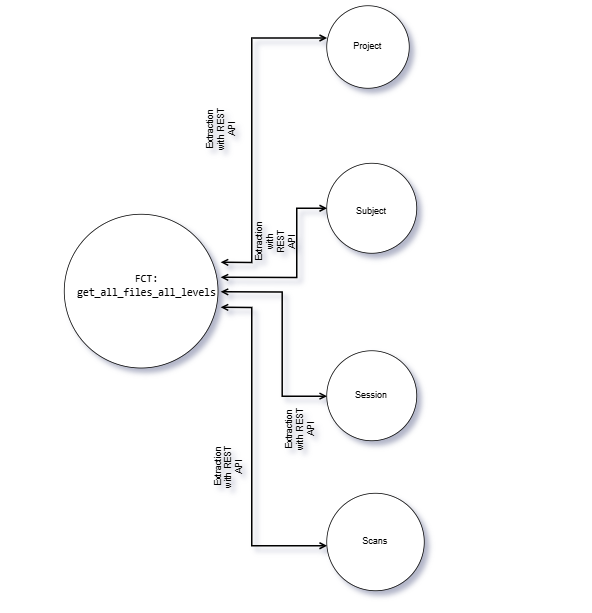
\includegraphics[width=0.6\linewidth]{en/content/edf.png}
    \caption{Diagram: The Extraction of files from all the project structure}
    \label{fig:enter-label}
\end{figure}




\section{Launch the Container:}
Arriving to the the famous we use the function \texttt{def launch\_container\_with\_all\_files}, this function is designed to automatically launch a container with all the files previously extracted as an input.It takes the XNAT server connection details, project and command identifiers, user authentication, the wrapper name, and a list of file to be processed. The function checks at the beginning if any file is provided. A payload dictionary is prepared, mapping the project ID and the input files string to the fields. The function next construct the appropriate URL for launching the command. Before sending the launch request, the function prints diagnostic information including the chosen files and payload, It submits a POST request with the payload as JSON and user credentials for authentication. After sending the request the Function report the user about the status and the responses.



\begin{lstlisting}
deflaunch_container_with_all_files(xnat_host,project_id,command_id,wrapper_name,xnat_user, xnat_password, files):
   
    if not files:
        print("no files found.")
        return 

    payload = {
        "project": project_id,
        "input_files": input_files_str
    }

    url = f"{xnat_host}/xapi/projects/{project_id}/commands/{command_id}/wrappers/{wrapper_name}/root/project/launch"

    headers = {"Content-Type": "application/json"}
    response = requests.post(
        url, auth=(xnat_user, xnat_password),
        headers=headers, json=payload, verify=False
    )

    print("Status:", response.status_code)
    print("Antwort:", response.text)
    if response.status_code in [200, 201, 202]:
        print("Container launched with all files!")
    else:
        print("failure :", response.status_code, response.text)
\end{lstlisting}



















